% This is a Basic Assignment Paper but with like Code and stuff allowed in it. 

\documentclass[11pt]{article}

% Preamble

\usepackage[margin=1in]{geometry}
\usepackage{amsfonts, amsmath, amssymb}
\usepackage{fancyhdr, float, graphicx}
\usepackage[utf8]{inputenc} % Required for inputting international characters
\usepackage[T1]{fontenc} % Output font encoding for international characters
\usepackage{fouriernc} % Use the New Century Schoolbook font
\usepackage[nottoc, notlot, notlof]{tocbibind}
\usepackage{listings}
\usepackage{xcolor}
\usepackage{float}

\definecolor{codegreen}{rgb}{0,0.6,0}
\definecolor{codegray}{rgb}{0.5,0.5,0.5}
\definecolor{codepurple}{rgb}{0.58,0,0.82}
\definecolor{backcolour}{rgb}{0.95,0.95,0.92}

\lstdefinestyle{mystyle}{
    backgroundcolor=\color{backcolour},   
    commentstyle=\color{codegreen},
    keywordstyle=\color{magenta},
    numberstyle=\tiny\color{codegray},
    stringstyle=\color{codepurple},
    basicstyle=\ttfamily\footnotesize,
    breakatwhitespace=false,         
    breaklines=true,                 
    captionpos=b,                    
    keepspaces=true,                 
    numbers=left,                    
    numbersep=5pt,                  
    showspaces=false,                
    showstringspaces=false,
    showtabs=false,                  
    tabsize=2
}

\lstset{style=mystyle}

% Header and Footer
\pagestyle{fancy}
\fancyhead{}
\fancyfoot{}
\fancyhead[L]{\textit{\Large{Computer Networks Assignment 10}}}
%\fancyhead[R]{\textit{something}}
\fancyfoot[C]{\thepage}
\renewcommand{\footrulewidth}{1pt}



% Other Doc Editing
% \parindent 0ex
%\renewcommand{\baselinestretch}{1.5}

\begin{document}
	
	\begin{titlepage} 
		\centering 
		
		%---------------------------NAMES-------------------------------
		
		\huge\textsc{
			MIT World Peace University
		}\\
	
		\vspace{0.75\baselineskip} % space after Uni Name
		
		\LARGE{
			Computer Networks\\
			Second Year B. Tech, Semester 3
		}
		
		\vfill % space after Sub Name
		
		%--------------------------TITLE-------------------------------
		
		\rule{\textwidth}{1.6pt}\vspace*{-\baselineskip}\vspace*{2pt}
		\rule{\textwidth}{0.6pt}
		\vspace{0.75\baselineskip} % Whitespace above the title
		
		
		
		\huge{\textsc{
			DHCP, DNS and Web Server configuration
			}} \\
		
		
		
		\vspace{0.5\baselineskip} % Whitespace below the title
		\rule{\textwidth}{0.6pt}\vspace*{-\baselineskip}\vspace*{2.8pt}
		\rule{\textwidth}{1.6pt}
		
		\vspace{1\baselineskip} % Whitespace after the title block

		%--------------------------SUBTITLE --------------------------	
			
		\LARGE\textsc{
			Practical Report\\
			Assignment 10
		} % Subtitle or further description
		\vfill
		
		%--------------------------AUTHOR-------------------------------
		
		Prepared By
		\vspace{0.5\baselineskip} % Whitespace before the editors
		
		\Large{
			Krishnaraj Thadesar \\
			Cyber Security and Forensics\\
			Batch A1, PA 20
		}
		
		
		\vspace{0.5\baselineskip} % Whitespace below the editor list
		\today

	\end{titlepage}
	
	
\tableofcontents
\thispagestyle{empty}
\clearpage


\setcounter{page}{1}

\section{Aim and Objectives}
\subsection*{Aim}
To Configure network using Dynamic Host Configuration Protocol (DHCP), DNS and Web server Use Ping utility to test connectivity.
\subsection*{Objectives}
\begin{enumerate}
	\item To learn the DHCP installation and understand the practical use of DHCP, DNS and Web server.
	\item To learn the mechanism to access the remote machine by using ping utility to test connectivity.
\end{enumerate}
\section{Devices}

\subsection{Devices Used}
\begin{enumerate}
	\item 1 Wireless Router WRT300N
	\item 1 Switch 2950
	\item 5 Generic PCs
	\item 3 Laptops
	\item 1 Web Server
\end{enumerate}

\subsection{Device Info and IP Addresses}

Subnet Mask: 255.255.255.0

\begin{table}[H] 
	\centering
	\begin{tabular}{|c|c|c|}
	\hline
	\textbf{Name} & \textbf{Type}      & \textbf{IP}    \\ 
	\hline
	PC0           & PC                 & 192.168.0.5   \\ 
	\hline
	PC1           & PC                 & 192.168.0.2   \\ 
	\hline
	PC2           & PC                 & 10.0.0.51   \\ 
	\hline
	PC3           & PC                 & 192.168.0.6   \\ 
	\hline
	PC6           & PC                 & 192.168.0.7   \\ 
	\hline
	Laptop0       & Laptop             & 192.168.0.3   \\ 
	\hline
	Laptop1       & Laptop             & 10.0.0.50   \\ 
	\hline
	\end{tabular}
	\end{table}

\section{Cables}
\begin{enumerate}
	\item Straight LAN Cable to connect unlike Devices
	\item Crossover LAN Cable to connect like Devices
\end{enumerate}

\section{Commands}
\begin{verbatim}
Router>enable
Router#config terminal
Router(config)#int fa0/0
Router(config-if)#ip add 192.168.1.1 255.255.255.0
Router(config-if)#no shutdown
Router(config-if)#exit
Router(config)#
Router(config)#ip dhcp pool MY_LAN
Router(dhcp-config)#network 192.168.1.0 255.255.255.0
Router(dhcp-config)#default-router 192.168.1.1
Router(dhcp-config)#dns-server 192.168.1.10
\end{verbatim}

\section{Theory}
\subsection{Dynamic Host Configuration Protocol (DHCP)}
\textit{The Dynamic Host Configuration Protocol (DHCP) is a network management protocol used on Internet Protocol (IP) networks for automatically assigning IP addresses and other communication parameters to devices connected to the network using a client-server architecture.}\\


Every device on a TCP/IP-based network must have a unique unicast IP address to access the network and its resources. Without DHCP, IP addresses for new computers or computers that are moved from one subnet to another must be configured manually; IP addresses for computers that are removed from the network must be manually reclaimed.\\


DHCP can be implemented on networks ranging in size from residential networks to large campus networks and regional ISP networks. Many routers and residential gateways have DHCP server capability. Most residential network routers receive a unique IP address within the ISP network. Within a local network, a DHCP server assigns a local IP address to each device.\\

DHCP services exist for networks running Internet Protocol version 4 (IPv4), as well as version 6 (IPv6). The IPv6 version of the DHCP protocol is commonly called DHCPv6.
\subsection{The Need for DHCP}
\begin{enumerate}
	\item On an IP network, each device connected to the Internet must be assigned a unique IP address. DHCP helps network administrators to monitor and assign IP addresses in a centralized manner.
	\item It can automatically assign a new IP address to a computer when it is moved to another location. DHCP automates the process of allocating IP addresses, which reduces the time required for device configuration and deployment, as well as the possibility of configuration errors. 
	\item A DHCP server can manage the configurations of multiple network segments. When the configuration of a network changes, an administrator only needs to update the corresponding configuration on the DHCP server.
\end{enumerate}
It Offers the Following Advantages:
\begin{enumerate}
	\item Reliable IP address configuration
	\item Reduced IP address conflicts
	\item Automatic IP address management
	\item Efficient change management
\end{enumerate}
\subsection{DHCP Message Format}
\begin{figure}[H]
	\centering
	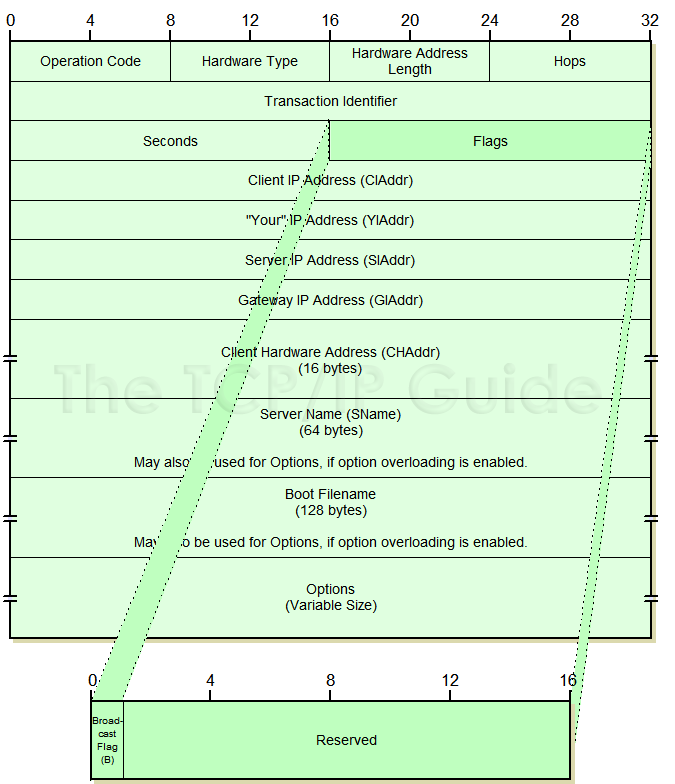
\includegraphics[scale = 0.8]{dhcpformat.png}
	\caption{The DHCP Message Format}
\end{figure}
\begin{itemize}
	\item \textit{Operation Code}:	Specifies the type of the Dynamic Host Configuration Protocol (DHCP) message. Set to 1 in messages sent by a client (requests) and 2 in messages sent by a server (response).
	\item \textit{Hardware}:  Type	Specifies the network LAN architecture. For example, the ethernet type is specified when htype is set to 1.
	\item \textit{Hardware}:  Address Length	Layer 2 (Data-link layer) address length (MAC address) (in bytes); defines the length of hardware address in the chaddr field. For Ethernet (Most widely used LAN Standard), this value is 6.
	Hops	Number of relay agents that have forwarded this message.
	\item \textit{Transaction}:  identifier	Used by clients to match responses from servers with previously transmitted requests.
	\item \textit{seconds}: 	Elapsed time (in seconds) since the client began theDynamic Host Configuration Protocol (DHCP) process.
	\item \textit{Flags}: 	Flags field is called the broadcast bit, can be set to 1 to indicate that messages to the client must be broadcast
	\item \textit{ciaddr}: 	Client's IP address; set by the client when the client has confirmed that its IP address is valid.
	\item \textit{yiaddr}: 	Client's IP address; set by the server to inform the client of the client's IP address.
	\item \textit{siaddr}: 	IP address of the next server for the client to use in the configuration process (for example, the server to contact for TFTP download of an operating system kernel).
	\item \textit{giaddr}: 	Relay agent (gateway) IP address; filled in by the relay agent with the address of the interface through which Dynamic Host Configuration Protocol (DHCP) message was received.
	\item \textit{chaddr}: 	Client's hardware address (Layer 2 address).
	\item \textit{sname}: 	Name of the next server for client to use in the configuration process.
	\item \textit{file}: 	Name of the file for the client to request from the next server (for example the name of the file that contains the operating system for this client).
\end{itemize}
\subsection{DHCP Operation}
The DHCP employs a connectionless service model, using the User Datagram Protocol (UDP). It is implemented with two UDP port numbers for its operations which are the same as for the bootstrap protocol (BOOTP). UDP port number 67 is the port used by the server, and UDP port number 68 is used by the client.\\

DHCP operations fall into four phases: server discovery, IP lease offer, IP lease request, and IP lease acknowledgement. These stages are often abbreviated as DORA for discovery, offer, request, and acknowledgement.

\begin{figure}[H]
	\centering
	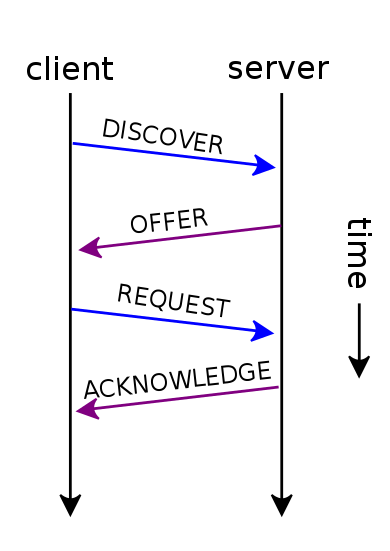
\includegraphics[scale = 0.4]{DHCP_session.svg.png}
	\caption{The DHCP Operations - DORA}
\end{figure}

\subsection{DNS and Email server}
DNS stands for Domain Name System or Domain Name Server. They are responsible for connecting domain names to web servers. Anytime you connect to the internet and go anywhere, you are using them.\\

The DNS records translate the domain into the IP address of the server that hosts it. The web server is then responsible for loading the site that matches the requested domain.

\subsubsection{SMTP AND DNS}
The \textbf{Domain Name System (DNS)} is a directory used by SMTP to convert a name, such as renovations.com, to a list of servers that can receive connections for that name and to find the IP address of a specific server. By looking up a destination server's address in the DNS, the sending server can properly route a message to a recipient.

DNS uses two kinds of records: \textbf{Mail Exchanger (MX)} records and A records. An MX record maps a domain name to the names of one or more mail hosts. An A record maps a host name to the IP address of a server.

Every email sent also generates a DNS lookup. And just like a domain name, each email address needs to map to an IP address
\begin{verbatim}
	User ID at domain name = info@example.com
\end{verbatim}

This format tells mail servers who and where the email should be delivered to. Without DNS, email could not function properly, which would be catastrophic for organizations that rely heavily on online correspondence.

Email runs on the following server types:
\begin{enumerate}
	\item \textbf{SMPT}: Simple Mail Transfer Protocol (SMPT) is used for outgoing mail and is part of the TCP/IP application layer. This protocol works with the Mail Transfer Agent (MTA) running on your mail server to ensure messages are sent to the proper address.
	\item \textbf{POP3}: Post Office Protocol, version 3 (POP3) is most commonly used for storing sent and received mail on local drives and/or servers. Once a user downloads the mail message, it is removed from the server.
	\item \textbf{IMAP}: Internet Message Access Protocol (IMAP) stores copies of messages on the server, rather than on a computer or device. This lets a user access files from emails from any device, as well as lets them organize mail without downloading beforehand.
\end{enumerate}
	\section{Procedure to Configure LAN}
\begin{enumerate}
	\item Create The network topology on the Packet tracer, that has a router, a few PCS near the router, and some connected to it via LAN cables. 
	\item Add a Web server which is connected to a switch that is connected to other end devices. 
	\item Run the commands on the router to configure it. 
	\item Go to the GUI tab in the router, and select the Wireless tab, where you can go to wireless security, and select security mode to WPA2, personal, and encryption to AE5. Assign a password. 
	\item To the PCs not connected to the router directly, install a wireless network card in them after turning them off, and then turn them back on. 
	\item Go the PC wireless in the Desktop Settings, and navigate to the Connect Tab. Here refersh the network, and add the WPA2 Passkey that you have assigned to the router. 
	\item To the webserver, add a Fast ethernet port to connect it. 
	\item Configure the Web Server, and add the Default gateway as 10.0.0.1
	\item Go to the services tab in the web server, and in DHCP, turn it on, and configure the starting and the ending IP addresses. Save. 
	\item Assign IP Addresses to all the other computers, by selecting on the DHCP Radiobutton instead of the static one, and wait for it to query and assign the IP. Ping and check. 
\end{enumerate}

\section{Platform}
	\textbf{Operating System}: Arch Linux x86-64\\
	\textbf{IDEs or Text Editors Used}: Visual Studio Code\\
	\textbf{Programs Used}: Cisco Packet Tracer v8.2

\section{Connection Screenshot}

\begin{figure}[H]
	\centering
	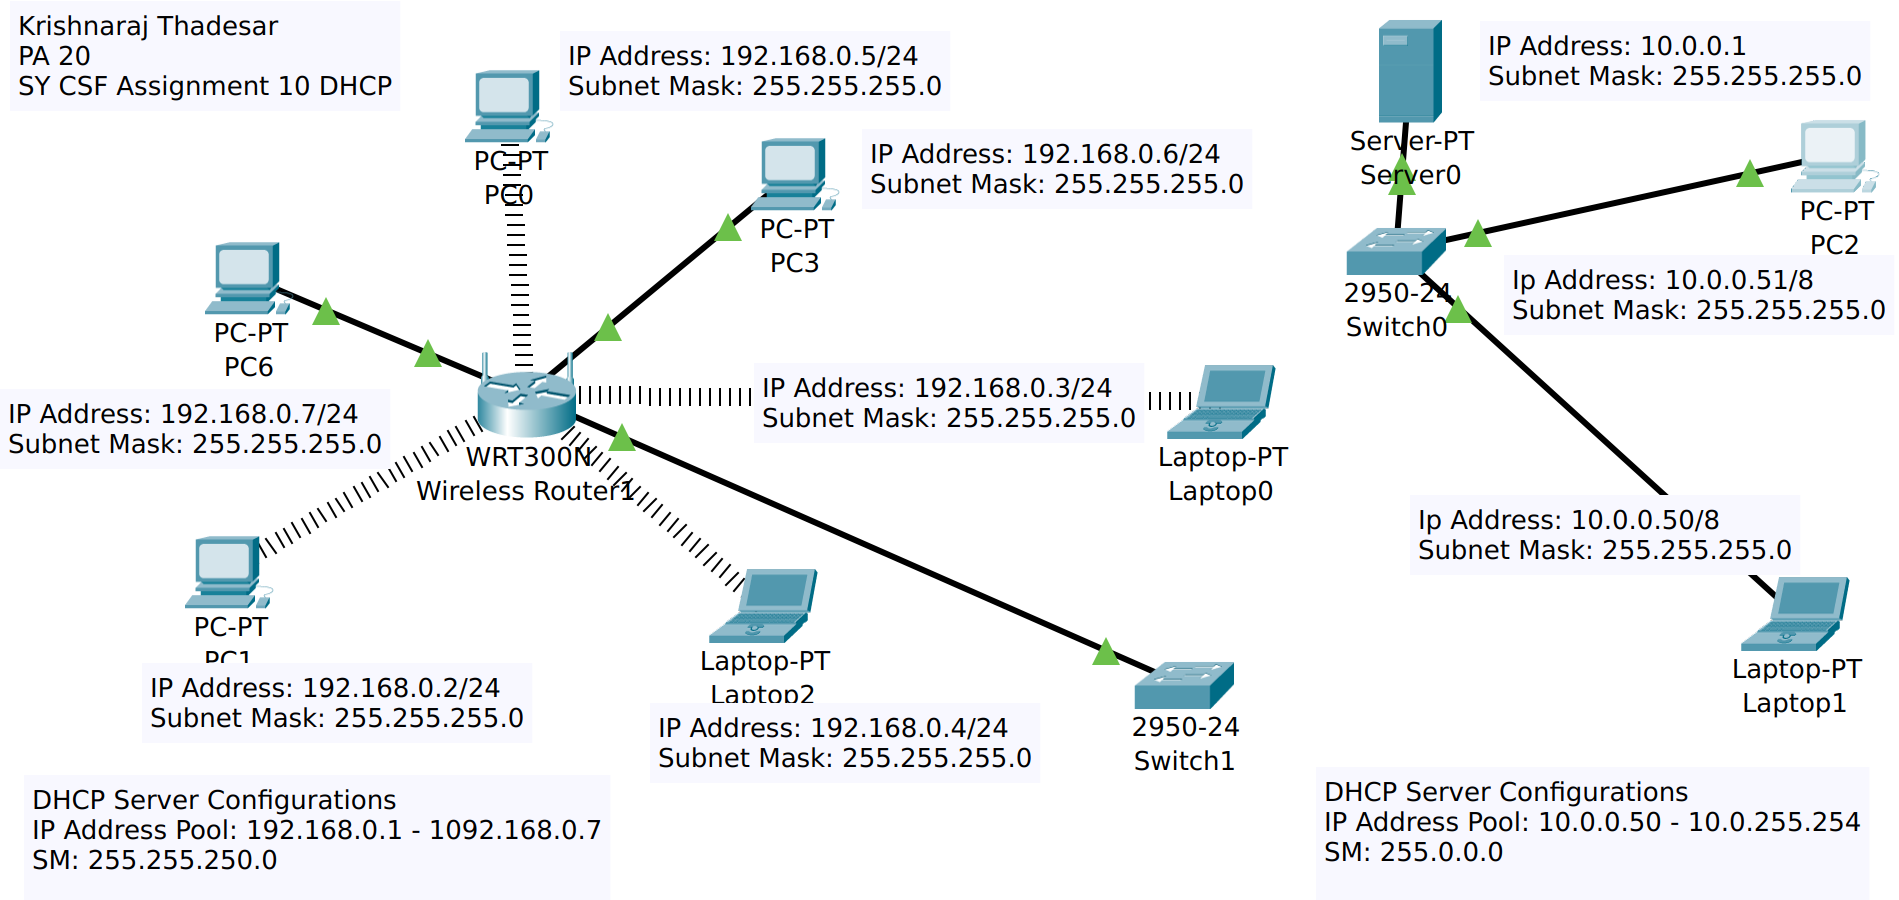
\includegraphics[scale=0.35]{../Screenshots/Assignment_10_screenshot.png}
\end{figure}


\section{Conclusion}
DHCP, DNS and Web Server configurations were implemented and understood successfully. 
\end{document}